\ProjectEntry
{EEG/EMG Vigilance Classification under Martian Photoperiod (T24.66)}
{First Student Author}
{EEG/EMG, FFT/Wavelet, Sleep \& Memory, Photoperiod}
{
  \bitem{Tested whether mammals adapt to Mars-like 12.33h light:12.33h dark cycles (T24.66).}
  \bitem{Found circadian realignment without free-running; ultradian noise increased under T24.66.}
  \bitem{Observed advanced siesta peak and increased midnight sleep; waking theta (8--12 Hz) attenuated at night.}
  \bitem{Night-time short-term object memory attenuated due to altered response to familiar objects; novelty response intact.}
}
{assets/1002_tamkwok/00_.png}
{\extlink{https://www.qqgjyx.com/files/p02-TamKwok-CNS2025.pdf}{CNS 2025 paper} \quad \extlink{https://qqgjyx.my.canva.site/s02-tamkwok-srs}{Slides}}
{\badge{CNN} \badge{PNAS Nexus under review} \badge{CNS 2025}}

\vspace{1em}

\textbf{Technical Highlights:}
We investigate mammalian adaptation to a Martian-length day (T24.66) using laboratory mice. The regime lengthens intrinsic period (\(\tau\)) enabling realignment to the slightly longer photoperiod without free running. Spectral analyses reveal preserved circadian power but amplified ultradian components; sleep architecture shifts and night-time waking theta decreases.

\begin{figure}[ht]
  \centering
  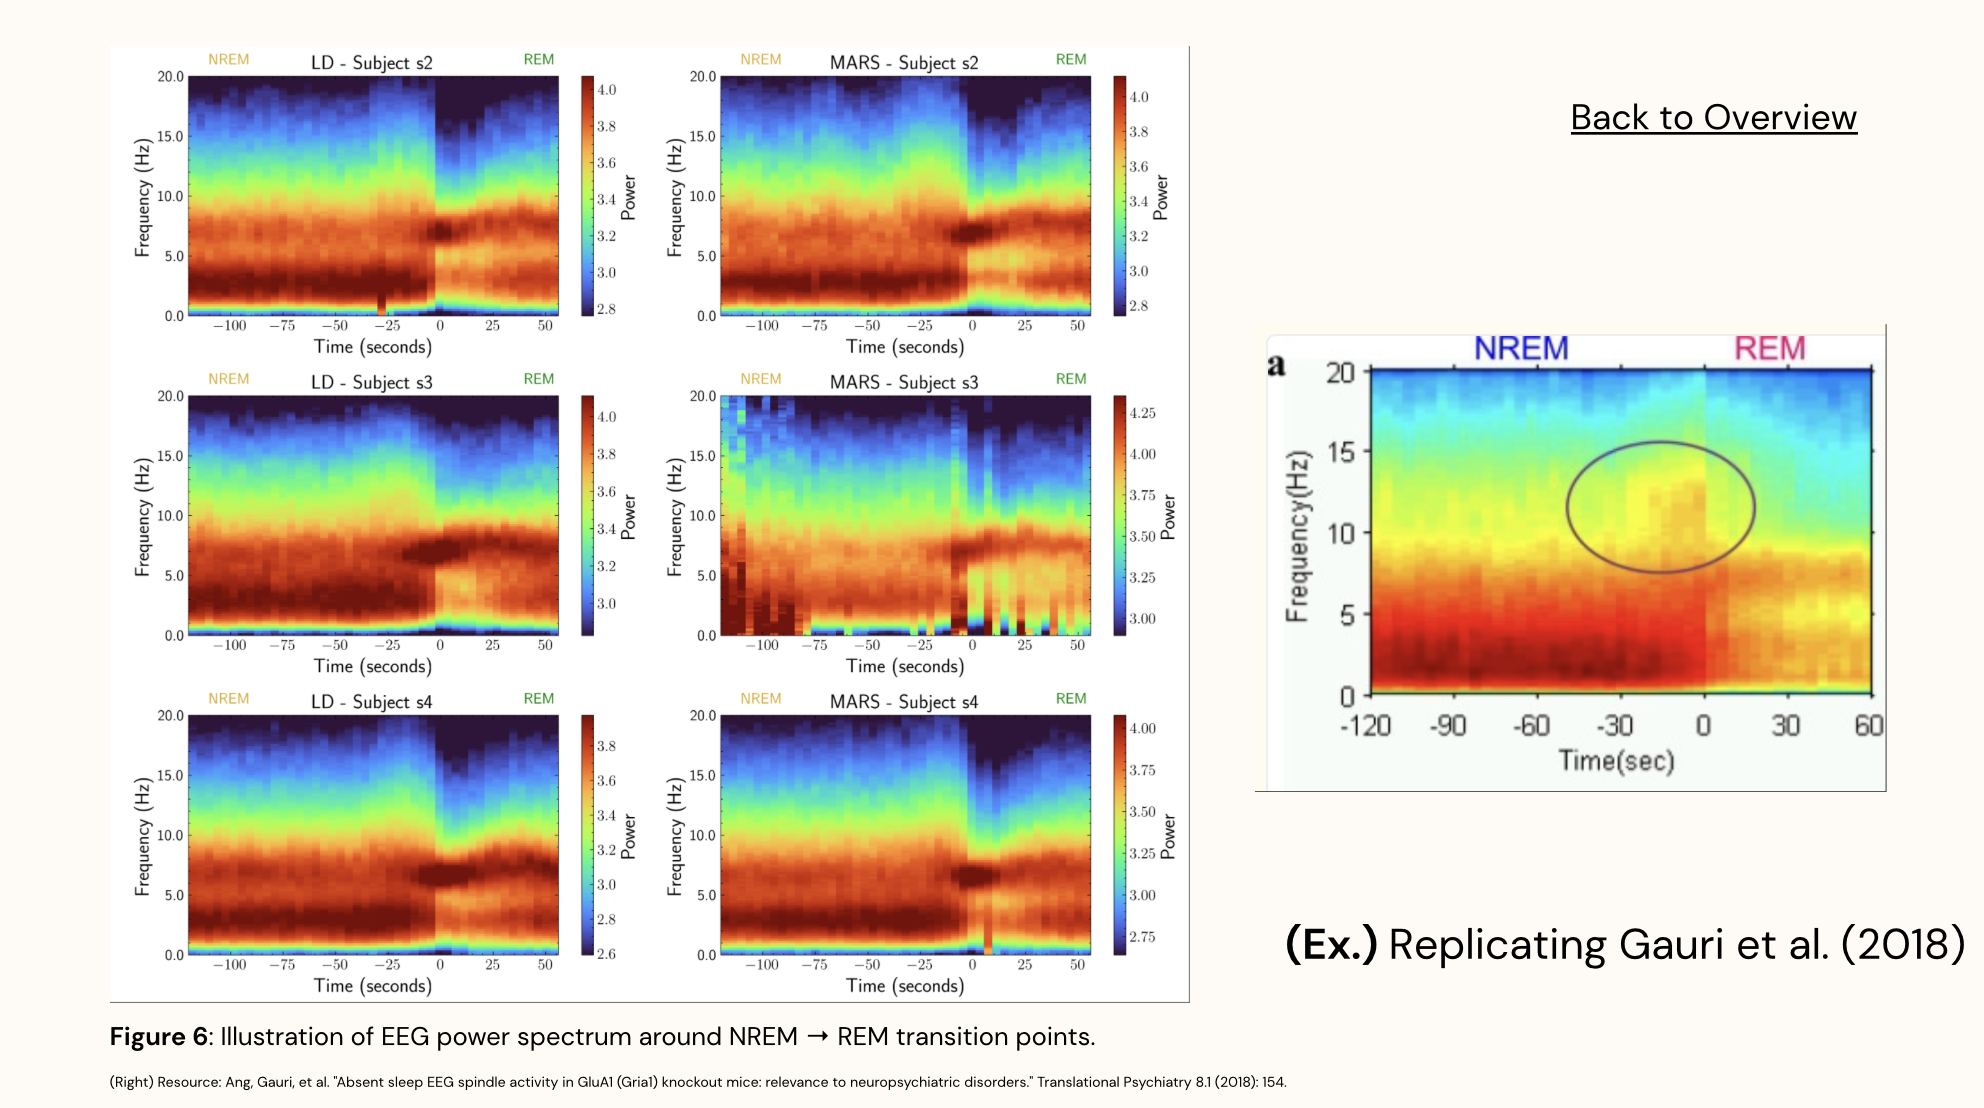
\includegraphics[width=0.85\linewidth]{assets/1002_tamkwok/01_.png}
  \caption{EEG spectral analyses around state transitions under T24.66. Wavelet/FFT-based spectra highlight attenuated waking theta (8--12 Hz) at night and altered sleep timing relative to T24.}
  \label{fig:t2466_spectra}
\end{figure}

\textbf{Methodology:}
\begin{itemize}[leftmargin=1.2em, itemsep=0.1em]
  \item Entrainment protocol: 12.33h light : 12.33h dark (T24.66) vs. T24 controls
  \item EEG/EMG recording; spectral analyses via fast Fourier transform (FFT) and wavelets
  \item Behavioral assessments: rest–activity rhythm, sleep timing, object memory assays
\end{itemize}

\textbf{Key Findings:}
\begin{itemize}[leftmargin=1.2em, itemsep=0.1em]
  \item Circadian: \(\tau\) lengthened; rhythms realigned with T24.66 without free running; circadian power not dampened
  \item Ultradian: Increased ultradian spectral power (FFT/wavelet)
  \item Sleep: Advanced siesta peak; increased midnight sleep; time-of-day dependent changes
  \item EEG: Night-time waking theta (8--12 Hz) attenuated
  \item Memory: Night-time short-term object memory attenuated due to altered response to familiar objects; novelty response spared
\end{itemize}

\textbf{Impact:} Findings suggest that adapting to a slightly non-24h photoperiod (T24.66) is feasible but entails neurophysiological trade-offs in sleep, alertness, and memory—relevant for space mission planning.

\vspace{1em}

\textbf{Publications:}
\begin{itemize}[leftmargin=1.2em, itemsep=0.1em]
  \item Shu Kit Eric Tam, Juntang Wang, Aleksandra Stryjska, Pascal Grange, Sze Chai Kwok. "Martian Photoperiod Attenuates Waking Theta Activity at Night and Disrupts Short-term Object Memory in Mice Despite Circadian Realignment." PNAS Nexus (under review).
  \item Shu Kit Eric Tam, Juntang Wang, Sze Chai Kwok. "Can the mammalian circadian system adapt to the Martian photoperiod?" Presented at CNS 2025.
\end{itemize}